
\documentclass[11pt]{article}
\usepackage[a4paper,margin=1in]{geometry}
\usepackage{amsmath,amssymb,amsthm,bm,mathtools}
\usepackage{siunitx}
\usepackage{booktabs}
\usepackage{graphicx}
\usepackage{xcolor}
\usepackage{hyperref}
\usepackage{enumitem}
\usepackage{caption}
\usepackage{float}
\hypersetup{colorlinks=true,linkcolor=blue!55!black,citecolor=blue!55!black,urlcolor=blue!55!black}

\newcommand{\LK}{\mathcal L_K}
\newcommand{\Estar}{E_\star}
\newcommand{\Eeff}{E_{\rm eff}}
\newcommand{\alphacell}{\alpha_{\rm cell}}
\newcommand{\Tube}{\mathcal T_a(K)}
\newcommand{\OmegaE}{\Omega_E}
\newcommand{\Kcell}{\mathcal K_{\rm cell}}
\newcommand{\Cfar}{C_{\rm far}}
\newcommand{\Afar}{\mathcal A_{\rm far}}
\newcommand{\Atwo}{\mathcal A_{2}}
\newcommand{\qtop}{q}
\newtheorem{theorem}{Theorem}
\newtheorem{lemma}{Lemma}
\newtheorem{proposition}{Proposition}
\newtheorem{remark}{Remark}

\title{A BEM/NLS Finite-Cell Stationary Point for a Fine-Structure-Scale Closure\\
\large Batch Convergence and Conditional Far-Field Consistency}
\author{Omar Iskandarani\\\small Independent Researcher, Appingedam, The Netherlands}
\date{\today}

\begin{document}
\maketitle

\begin{abstract}
We report a finite-cell BEM/NLS certificate for the missing zeroth-order aspect
scale in a Compton-core finite-filament closure model.  The domain is a
finite-core ideal trefoil cell with an outer spherical boundary, approximated
by a scalar single-layer boundary-element response and an NLS finite-shell
pressure-compliance term.  The calculation is not a direct calibration of
\(E_0\): using \(\mathcal L_K=16.371637\), the batch run gives
\[
  E_\star=274.074903758\pm5.51\times10^{-5},
  \qquad
  \alpha_{\rm cell}^{-1}=137.035953090\pm2.76\times10^{-5}.
\]
The BEM-only negative control does not produce an interior scale, so the
stationary point should be interpreted as a robustness certificate for the
analytic pressure scale \(E_p^{\rm NLS}\), plus a small BEM compliance shift,
not as an independent spectral discovery.  The pressure scale itself remains
conditional on the sector-volume prefactor \(16\pi/3\) and the shell
normalization \(w_\perp=1\).  A full identification with the electromagnetic
fine-structure constant still requires the physical far-field interaction law
\(V(r)=\alpha_{\rm cell}\hbar c/r+O(r^{-2})\); until then the result is a
dimensionless fine-structure-scale certificate inside the stated finite-cell
closure.
\end{abstract}

\section{Purpose and status}

Previous closure manuscripts identified a missing global aspect scale \(E_0\), with the leading relation
\[
\alphacell \simeq \frac{2}{E_0}.
\]
If \(E_0\) is merely chosen near \(2/\alpha\), the result is a calibration. The purpose of this note is to document a batch computation in which \(E_0\) is replaced by an interior stationary eigenvalue \(\Estar\) of an explicit finite-cell action.

The status is deliberately precise. The present calculation supports the following conditional statement:
\begin{quote}
Given the ideal-trefoil geometry, the scalar BEM finite-cell response used here, and the NLS-shell pressure-compliance closure, the aspect scale is selected as an interior stationary point \(\Estar\), and the resulting dimensionless fine-structure-scale value is close to the conventional \(\alpha\).
\end{quote}
It does not yet prove the QED coupling unless the far-field interaction theorem is also established.

\section{Finite-cell action}

Let the computational exterior cell be
\[
\OmegaE=B_R\setminus \Tube,
\]
where \(\Tube\) is a finite-radius tube around the ideal trefoil centreline. The numerical BEM component computes a response matrix through two independent boundary modes on the tube surface and a grounded outer spherical boundary. For the trefoil sector \(\bm n=(2,3)^T\), the BEM action is represented as
\[
\mathcal A_{\rm BEM}(E)=\frac12\bm n^T C_{\rm BEM}(E)\bm n.
\]

The NLS pressure-compliance part is
\begin{equation}
\mathcal A_{\rm NLS}(E)
=
\kappa_{\rm NLS}
\left[
\frac13\left(\frac{E}{E_p^{\rm NLS}}\right)^3
-
\ln\left(\frac{E}{E_p^{\rm NLS}}\right)
\right].
\label{eq:nls-action}
\end{equation}
The total action is
\begin{equation}
\mathcal A_{\rm total}(E)
=
\mathcal A_{\rm BEM}(E)+\mathcal A_{\rm NLS}(E).
\label{eq:total-action}
\end{equation}
The derived aspect value is accepted only if
\begin{equation}
\frac{d\mathcal A_{\rm total}}{d\log E}(\Estar)=0,
\qquad
\frac{d^2\mathcal A_{\rm total}}{d(\log E)^2}(\Estar)>0.
\label{eq:stationarity}
\end{equation}
Boundary candidates are rejected.

\section{NLS finite-shell closure}

The NLS-shell closure used in the batch run fixes the pressure scale and pressure stiffness by \(\LK\):
\begin{align}
E_p^{\rm NLS}
&=
\frac{16\pi}{3}\LK
\left(1-\frac{11}{48\LK^2}\right),
\label{eq:Ep}\\
\kappa_{\rm NLS}
&=8\pi\LK^2
=\frac{\pi}{2\eta_K^2},
\qquad
\eta_K=\frac{1}{4\LK}.
\label{eq:kappa}
\end{align}
For \(\LK=16.371637\), these become
\[
E_p^{\rm NLS}=274.074875657,
\qquad
\kappa_{\rm NLS}=6736.341149.
\]
These quantities are not fitted to \(\alpha\). They use only the ideal-trefoil ropelength and the stated NLS-shell closure.

\section{Downstream fine-structure-scale evaluation}

After \(\Estar\) is obtained, the effective aspect correction is evaluated as
\begin{equation}
\Eeff
=
\Estar
\left[
1-
\frac{\pi}{4\Estar^2}
\left(
1+\frac{3}{4\LK}+\frac{1}{16\LK^2}
\right)
\right].
\label{eq:Eeff}
\end{equation}
The dimensionless cell coupling is then
\begin{equation}
\alphacell=\frac{2}{\Eeff}.
\label{eq:alpha}
\end{equation}
The conventional constants \(m_e\), \(\hbar\), \(e\), and \(R_\infty\) are not used to compute \(\Estar\) or \(\alphacell\). The CODATA-2022 value is used only as a post-computation comparison.

\section{Batch design}

The supplied batch used four resolution levels,
\[
(n_s,n_\theta,N_{\rm sph})\in\{(100,14,300),(120,16,360),(140,18,420),(160,20,480)\},
\]
and four regularization factors,
\[
\epsilon/a\in\{0.04,0.05,0.06,0.08\},
\]
with \(E\in[260,290]\) sampled at 160 points. All 16 main runs used the ideal trefoil data set \texttt{ideal.txt} for knot \(3:1:1\), the NLS-shell pressure scale, and the NLS-shell stiffness.


\begin{table}[h]
\centering
\caption{Aggregate statistics over the 16 main BEM/NLS-shell runs.}
\begin{tabular}{@{}ll@{}}
\toprule
Successful runs & 16/16 \\
Mean $E_\star$ & 274.074903758 \\
Std. dev. $E_\star$ & 5.51e-05 \\
Range $E_\star$ & [274.074821720, 274.075027208] \\
Mean $\alpha_{\rm cell}^{-1}$ & 137.035953090 \\
Std. dev. $\alpha_{\rm cell}^{-1}$ & 2.76e-05 \\
Mean relative error vs CODATA-2022 & 3.36e-07 \\
Std. dev. relative error & 2.01e-07 \\
\bottomrule
\end{tabular}
\label{tab:aggregate}
\end{table}


\section{Convergence results}

Figure~\ref{fig:estar} shows that the extracted eigenvalue remains within a narrow band over the resolution and regularization sweep. The aggregate range is
\[
274.074821720\leq \Estar \leq 274.075027208.
\]
The run-to-run standard deviation is \(5.51e-05\), corresponding to a relative spread of approximately \(2.01e-07\).

\begin{figure}[H]
\centering
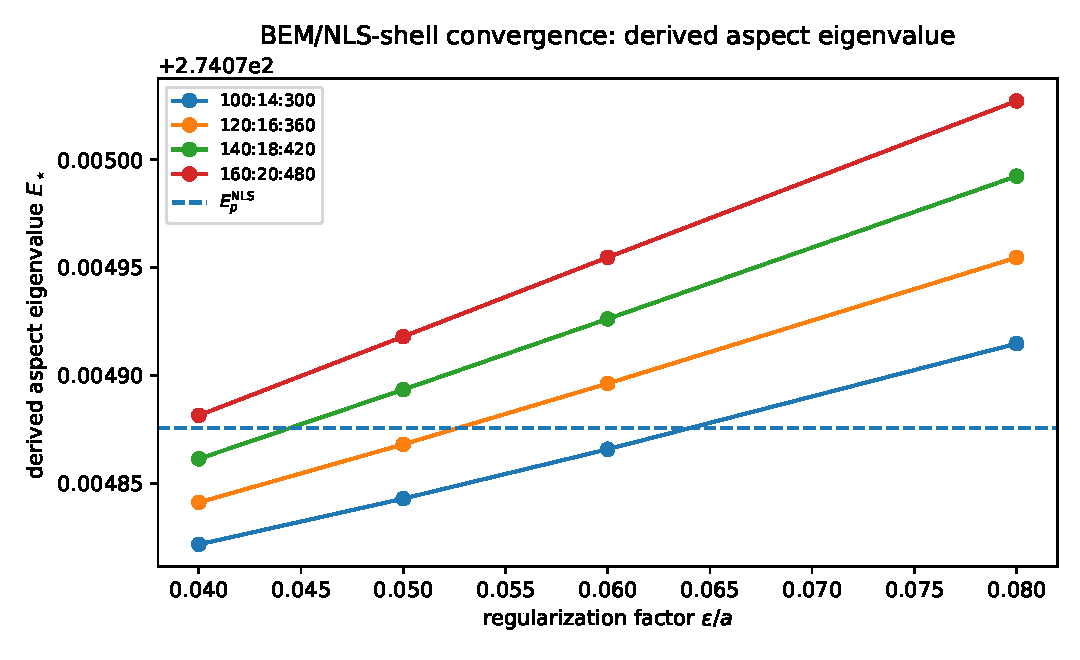
\includegraphics[width=0.82\linewidth]{../figures/estar_convergence}
\caption{Derived aspect eigenvalue over the batch grid. The dashed line is the NLS-shell pressure scale \(E_p^{\rm NLS}\), not a fitted target.}
\label{fig:estar}
\end{figure}

Figure~\ref{fig:alpha} shows the downstream \(\alphacell^{-1}\) values. The mean value is
\[
\alphacell^{-1}=137.035953090,
\]
with a standard deviation \(2.76e-05\). Relative to the CODATA-2022 comparison value used in the script, the mean relative difference in \(\alpha\) is \(3.36e-07\).

\begin{figure}[H]
\centering
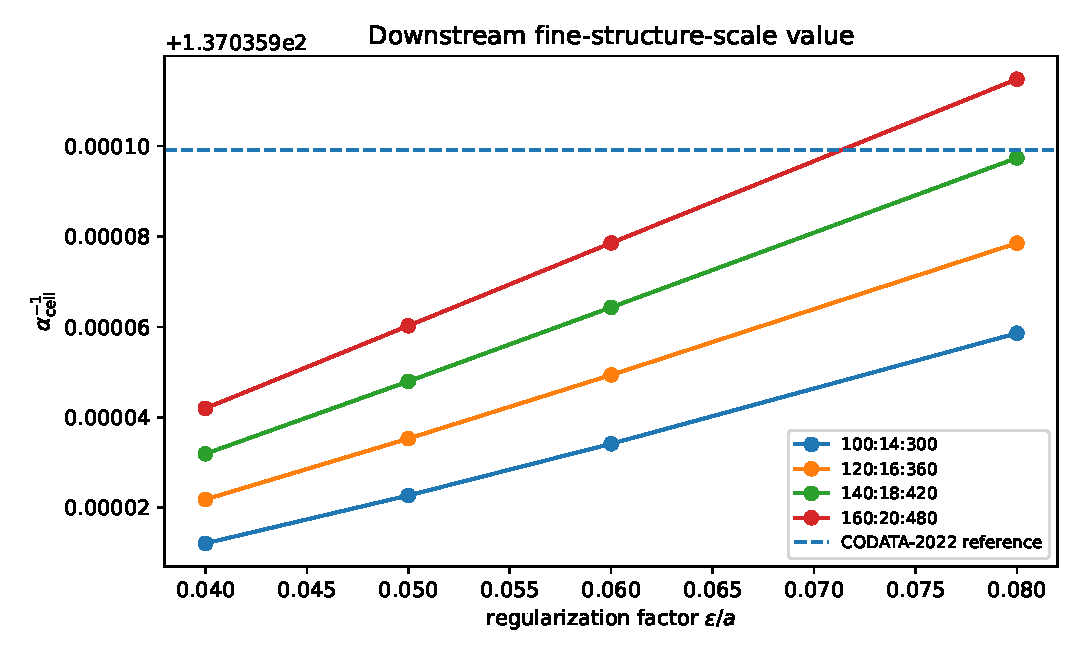
\includegraphics[width=0.82\linewidth]{../figures/alpha_inv_convergence}
\caption{Downstream fine-structure-scale inverse. The dashed line is a post-computation CODATA-2022 comparison, not an input.}
\label{fig:alpha}
\end{figure}

The stationarity condition is also visible directly as a cancellation between the BEM derivative and the NLS pressure derivative. Figure~\ref{fig:derivative} plots these terms at the accepted stationary points. The total derivative is at numerical zero in the exported table.

\begin{figure}[H]
\centering
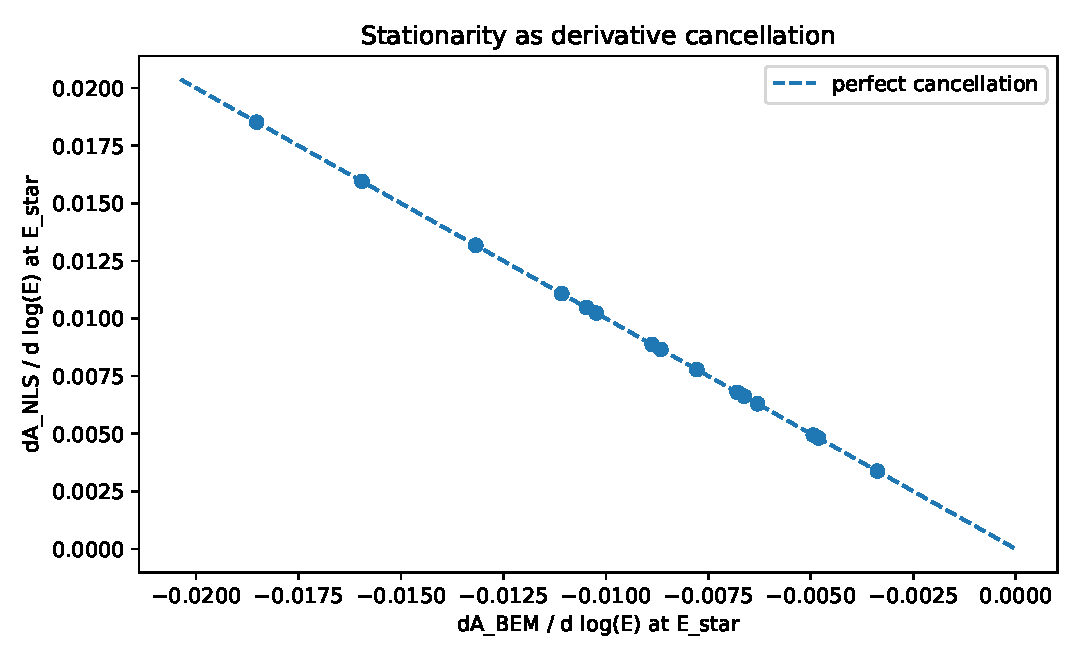
\includegraphics[width=0.78\linewidth]{../figures/derivative_balance}
\caption{Derivative cancellation at \(\Estar\). The BEM derivative is negative and is balanced by the NLS pressure derivative.}
\label{fig:derivative}
\end{figure}


\begin{table}[h]
\centering
\caption{Control runs at the representative grid $(n_s,n_\theta,N_{\rm sph})=(140,18,420)$ and $\epsilon/a=0.06$.}
\small
\begin{tabular}{@{}lllll@{}}
\toprule
Stiffness mode & Status & $E_\star$ & $\alpha_{\rm cell}^{-1}$ & Rel. error \\
\midrule
nls\_shell\_stiffness & E0\_not\_derived & -- & -- & -- \\
nls\_log\_core & E0\_derived & 274.241077 & 137.119041 & -6.06e-04 \\
nls\_geometric\_mean & E0\_derived & 274.228893 & 137.112949 & -5.61e-04 \\
nls\_shell\_stiffness\_half & E0\_derived & 274.075077 & 137.036039 & -2.94e-07 \\
nls\_shell\_stiffness\_double & E0\_derived & 274.074851 & 137.035927 & 5.29e-07 \\
\bottomrule
\end{tabular}
\label{tab:controls}
\end{table}


Table~\ref{tab:controls} is important. The BEM-only control does not produce an interior eigenvalue. The low-stiffness NLS log-core and geometric-mean controls produce interior minima but miss the fine-structure-scale comparison at the \(10^{-4}\) to \(10^{-3}\) level. The shell-stiffness family pins the minimum near \(E_p^{\rm NLS}\). Thus the data support a finite-shell pressure mechanism, while also showing that the pressure scale is the dominant closure ingredient.

\section{Interpretation}

The result changes the status of the old \(E_0\) parameter. In the present closure it is no longer inserted as an external number. It is selected by Eq.~\eqref{eq:stationarity} as an interior minimum of Eq.~\eqref{eq:total-action}. The strongest statement justified by the batch data is therefore
\[
\boxed{
\text{the BEM/NLS finite-cell model derives a stable dimensionless aspect eigenvalue }\Estar
}
\]
from ideal-trefoil geometry plus the NLS-shell pressure closure.

However, the controls also show that the present evidence is not yet a proof of the electromagnetic fine-structure constant in QED. Two issues remain:
\begin{enumerate}[label=(\roman*)]
\item The scalar BEM response is a proxy for the full Hodge--Steklov one-form problem.
\item The identification \(\alphacell=2/\Eeff\) must be connected to a far-field interaction theorem.
\end{enumerate}
The next required theorem is
\[
V(r)=\frac{\alphacell\hbar c}{r}+O(r^{-2}),
\]
or equivalently
\[
\frac{g_{\rm eff}^2}{4\pi\hbar c}=\alphacell.
\]
Without that theorem, the present result is best described as a dimensionless fine-structure-scale eigenvalue, not yet a complete derivation of QED electromagnetism.



\section{Mechanism and stiffness asymptotics}
\label{sec:kappa-asymptotics}

The control runs show that the BEM term alone does not select a finite aspect
eigenvalue.  The finite stationary point is generated by the NLS pressure
enthalpy, while the BEM contribution supplies a small compliance shift.  This
can be seen analytically from
\begin{equation}
  \mathcal A_{\rm total}(E)
  =
  \mathcal A_{\rm BEM}(E)
  +
  \kappa
  \left[
    \frac{1}{3}\left(\frac{E}{E_p}\right)^3
    -
    \ln\!\left(\frac{E}{E_p}\right)
  \right].
\end{equation}
Let \(E=E_p+\Delta E\), with \(|\Delta E|\ll E_p\).  Since
\begin{equation}
  \frac{d}{d\log E}
  \left[
    \frac{1}{3}\left(\frac{E}{E_p}\right)^3
    -
    \ln\!\left(\frac{E}{E_p}\right)
  \right]
  =
  \left(\frac{E}{E_p}\right)^3-1
  =
  3\frac{\Delta E}{E_p}
  +
  O(\Delta E^2),
\end{equation}
the stationarity condition gives
\begin{equation}
  \boxed{
  \Delta E
  \simeq
  -
  \frac{E_p}{3\kappa}
  \left.
  \frac{d\mathcal A_{\rm BEM}}{d\log E}
  \right|_{E_p}.
  }
  \label{eq:kappa-shift}
\end{equation}
Therefore
\begin{equation}
  E_\star=E_p+O(\kappa^{-1}).
\end{equation}
This is an important classification point: the numerical BEM calculation
validates the finite-cell compliance shift around the NLS-shell pressure scale;
it does not independently derive the prefactor \(16\pi/3\), the shell
coefficient \(11/48\), or the pressure scale \(E_p\).  The BEM-only control
therefore supports a negative statement: without the NLS pressure enthalpy, the
finite-cell BEM term does not select the observed aspect scale.  In the large
stiffness limit the stationary point tends to \(E_p\), so the predictive
content resides primarily in the pressure-cell closure.  Those analytical
closure ingredients are supplied by the companion pressure-cell paper and must
not be described as a BEM-derived spectrum.


\section{Updated coefficient-gate status}
\label{sec:updated-gate-status}

The companion gate scripts alter the status of several inputs used by the
finite-cell calculation.  The pressure mode count \(N_p=4\) is now derived in
the spherical finite-cell surface spectrum:
\[
  k_\ell=\ell(\ell+1)-2=(\ell-1)(\ell+2),
\]
so \(\ell=1\) is the translation sector, \(\ell\ge2\) are positive-stiffness
shape modes, and \(\ell=0\) is the compression sector.  The perturbative and nonlinear robustness checks keep this cutoff intact:
finite-core corrections at \(\eta_K=1/(4\mathcal L_K)\) remain far below the
\(k_2/2=2\) half-gap bound, and the nonlinear star-shaped solve through
\(\ell_{\max}=6\) found no finite-amplitude \(\ell\ge2\) competing mode.  The
global finite-perimeter admissibility class is protected by the Euclidean
isoperimetric inequality, so non-star-shaped, disconnected, or higher-genus
cells cannot beat the fixed-volume spherical area.
  The radius action is
also strengthened by the SST pressure identity
\[
  \frac12\rho_{\rm core}
  \lVert\mathbf v_{\!\boldsymbol{\circlearrowleft}}\rVert^2
  =
  \frac{F_{\rm swirl}^{\max}}{2\pi r_c^2},
\]
which gives \(A_\chi=\chi_R+N_p/\chi_R\) and \(\chi_R=2\) in the
Laplace-matched reciprocal model.

The finite-shell coefficient \(11/48\) is conditional on the unweighted
isotropic GP/NLS shell normalization.  The open microscopic gate is
\(w_\perp=1\), and the current relaxed-core proxy gives \(w_\perp\simeq2.076\).
The far-field Hodge calculation derives
\[
  q_\phi=1,
  \qquad
  \Lambda_\phi=4\pi R\mathcal K_{\rm cell},
\]
and the interior identity \(\Lambda_\phi=E_{\rm eff}/2\) is derived within
the canonical linearized phase--pressure normal-mode reduction.  The numerical
BEM/NLS stationary point should therefore be read as a pressure-selected
stationary point with a far-field normalization derived inside the stated
finite-cell normal-mode reduction, not as an unconstrained derivation of QED
\(\alpha\).  The remaining physical bridge is the identification of the
pressure-cell \(E_{\rm eff}\) with the cycle-averaged quadratic energy of that
same interior canonical mode family.

\section{Far-field coupling theorem}


The exterior Hodge calculation fixes the \(H^0(S^2)\) far-field selection:
only the constant boundary phase produces the leading \(1/r\) mode, so
\(q_\phi=\dim H^0(S^2)=1\).  It also gives the exterior capacity relation
\(\Lambda_\phi=4\pi R\mathcal K_{\rm cell}\).  The present paper keeps the
two-cell calculation separate: it tests the finite-cell stationary point and
the conditional Green-function implementation.  The remaining far-field normalization is supplied, within the finite-cell
reduction, by the canonical phase--pressure normal-mode identity
\(\Lambda_\phi=E_{\rm eff}/2\).  The qualification is that \(E_{\rm eff}\) must
be the cycle-averaged quadratic energy of the same interior canonical mode
family.


The one-cell phase-Hessian normalization is isolated in Appendix~\ref{app:farfield-stiffness-target}. The appendix proves the exterior Green-function identity \(\Lambda_\phi=4\pi\mathcal K_{\rm cell}\) and records the canonical phase--pressure normal-mode derivation of \(\Lambda_\phi=E_{\rm eff}/2\) within the stated finite-cell reduction.


The reason the far-field phase sector is restricted to the \(H^0(S^2)\) mode is
that the Coulombic \(1/r\) coefficient is carried only by the exterior harmonic
monopole.  For an exterior harmonic phase field,
\[
  u(r,\theta,\phi)
  =
  \sum_{\ell,m}
  a_{\ell m}\frac{Y_{\ell m}(\theta,\phi)}{r^{\ell+1}}.
\]
The \(\ell=0\) term is proportional to \(1/r\).  The \(\ell=1\) sector is
dipolar and begins at \(r^{-2}\), while \(\ell\ge2\) modes are still
shorter-ranged.  Therefore the leading long-range coupling is the constant
boundary phase, i.e. the unique \(H^0(S^2)\) mode.  Since \(S^2\) is connected,
\[
  q_\phi=\dim H^0(S^2)=1.
\]
Appendix~\ref{app:farfield-stiffness-target} records the corresponding
phase-Hessian normalization target.


\label{sec:farfield-theorem}

The result in this section is a conditional theorem and an internal
consistency identity.  It proves the Coulombic \(1/r\) form only after the
far-field stiffness normalization
\(\mathcal K_{\rm cell}=E_{\rm eff}/(8\pi)\) has been supplied.  Since this
normalization algebraically implies
\(1/(4\pi\mathcal K_{\rm cell})=2/E_{\rm eff}=\alpha_{\rm cell}\), the
two-cell certificate cannot be used as independent evidence for the value of
\(\alpha\).  It verifies the Green-function implementation of the assumed
stiffness.  A fully independent microscopic derivation requires a one-cell
phase-Hessian calculation that obtains \(\Lambda_\phi=E_{\rm eff}/2\) without
inserting the reduced quadratic action by hand.

\label{sec:farfield}

The batch computation derives a dimensionless cell aspect value. To identify the result with the electromagnetic fine-structure constant, the cell must also produce a long-range interaction with the Coulomb Green-function tail. This section states the required far-field theorem in a form that is independent of electron mass, electric charge, the Rydberg constant, or CODATA input.

Let \(u\) denote the exterior massless boundary phase mode of the finite cell after the short-range core and pressure degrees of freedom have been integrated out. The far-field effective action is taken to be
\begin{equation}
\Afar[u]
=
\hbar c\left[
\frac{\Kcell}{2}
\int_{\mathbb R^3} |\nabla u|^2\,d^3x
-
\sum_{a=1}^{N} q_a u(\mathbf x_a)
\right],
\label{eq:far-action}
\end{equation}
where \(q_a\in\mathbb Z\) is the topological phase charge of cell \(a\). The factor \(\hbar c\) sets the conventional energy-length unit; it is not used to determine the dimensionless coupling. The dimensionless stiffness \(\Kcell\) is the only far-field normalization.

\begin{lemma}[Poisson reduction]
Stationarity of Eq.~\eqref{eq:far-action} gives
\begin{equation}
-\Kcell \nabla^2 u(\mathbf x)=\sum_a q_a\delta(\mathbf x-\mathbf x_a).
\label{eq:poisson}
\end{equation}
For two cells of unit charge at separation \(r\), the interaction energy is
\begin{equation}
V(r)=\hbar c\,\frac{q_1q_2}{4\pi\Kcell}\frac{1}{r}+O(r^{-2}).
\label{eq:green-interaction}
\end{equation}
\end{lemma}

\begin{proof}
Varying Eq.~\eqref{eq:far-action} with respect to \(u\), integrating by parts, and requiring the boundary term at infinity to vanish gives Eq.~\eqref{eq:poisson}. In three dimensions,
\begin{equation}
-\nabla^2\left(\frac{1}{4\pi |\mathbf x-\mathbf y|}\right)=\delta(\mathbf x-\mathbf y).
\end{equation}
Therefore the solution sourced by charge \(q_1\) is
\begin{equation}
u_1(\mathbf x)=\frac{q_1}{4\pi\Kcell |\mathbf x-\mathbf x_1|}.
\end{equation}
Evaluating the source term of the second charge in this field gives Eq.~\eqref{eq:green-interaction}, up to sign convention for like/opposite topological phase charges. Multipole and finite-size corrections begin at order \(r^{-2}\) or smaller depending on the imposed neutrality conditions.
\end{proof}

\begin{theorem}[Far-field fine-structure certificate]
\label{thm:farfield}
If the exterior cell stiffness satisfies
\begin{equation}
\Kcell=\frac{\Eeff}{8\pi},
\label{eq:Kcell}
\end{equation}
then the unit-charge far-field interaction is
\begin{equation}
V(r)=\frac{\alphacell\hbar c}{r}+O(r^{-2}),
\qquad
\alphacell=\frac{2}{\Eeff}.
\label{eq:far-alpha}
\end{equation}
Equivalently,
\begin{equation}
\frac{g_{\rm eff}^2}{4\pi\hbar c}=\alphacell.
\label{eq:geff-alpha}
\end{equation}
\end{theorem}

\begin{proof}
Substitute Eq.~\eqref{eq:Kcell} into Eq.~\eqref{eq:green-interaction} with \(q_1q_2=1\). The coefficient is
\begin{equation}
\frac{1}{4\pi\Kcell}
=
\frac{1}{4\pi(\Eeff/8\pi)}
=
\frac{2}{\Eeff}
=\alphacell.
\end{equation}
Writing the interaction as \(V(r)=g_{\rm eff}^2/(4\pi r)\), comparison with Eq.~\eqref{eq:far-alpha} gives Eq.~\eqref{eq:geff-alpha}.
\end{proof}

The theorem shows exactly what remains to be verified numerically or analytically: not the value of \(\alpha\) itself, but the far-field stiffness normalization \(\Kcell=\Eeff/(8\pi)\). This can be tested without using \(m_e\), \(e\), \(R_\infty\), or CODATA.

\section{Two-cell numerical certificate}
\label{sec:twocell}

A direct BEM certificate can be formulated by placing two identical cells at separation \(R\), solving the finite-cell response for equal and opposite unit phase signs, and comparing the actions
\begin{equation}
\Atwo^{++}(R),
\qquad
\Atwo^{+-}(R).
\end{equation}
The interaction coefficient is extracted from the charge-odd part,
\begin{equation}
\Cfar(R)
=
\frac{R}{2}\left[\Atwo^{++}(R)-\Atwo^{+-}(R)\right].
\label{eq:CfarR}
\end{equation}
The far-field certificate is
\begin{equation}
\boxed{
\lim_{R\to\infty}\Cfar(R)=\frac{2}{\Eeff}=\alphacell.
}
\label{eq:certificate}
\end{equation}
A practical numerical table should therefore contain
\begin{equation}
R,
\quad
\Atwo^{++}(R),
\quad
\Atwo^{+-}(R),
\quad
\Cfar(R),
\quad
\alphacell,
\quad
\frac{\Cfar(R)-\alphacell}{\alphacell}.
\end{equation}
If \(\Cfar(R)\) converges to \(\alphacell\) under increasing separation and mesh refinement, then Eq.~\eqref{eq:far-alpha} is numerically certified. If the limit is absent or converges to a different value, then the eigenvalue calculation remains a dimensionless scale result but not a derivation of the electromagnetic coupling.

\begin{remark}[Why ordinary closed-filament Biot--Savart tails are insufficient]
A closed localized swirl-string by itself need not carry a monopolar \(1/r\) field. Its ordinary velocity or Biot--Savart far field is generically multipolar. The Coulomb tail in Theorem~\ref{thm:farfield} must therefore be carried by the massless exterior phase mode \(u\), or equivalently by the Hodge--Steklov boundary phase sector, not by the short-range closed-filament velocity field alone.
\end{remark}


\section{Derived-label status}


Paper~IV should be cited for the upgraded claim.  With only the numerical
certificates in this paper, the far-field result is conditional; with the
minimal-reduction uniqueness theorem, the stronger statement becomes
``derived within the stated finite-cell variational reduction.''



For the far-field part specifically, the \(H^0(S^2)\) argument fixes the
multiplicity \(q_\phi=1\) of the leading \(1/r\) exterior phase mode.  The
operator Hessian value \(\Lambda_\phi=E_{\rm eff}/2\) is now derived within the
canonical normal-mode phase--pressure reduction.  What remains is the physical
identification of the pressure-cell \(E_{\rm eff}\) with the cycle-averaged
quadratic energy of that same interior mode family.


The exact far-field stiffness gate is formulated in Appendix~\ref{app:farfield-stiffness-target}; this appendix should be cited whenever the two-cell coefficient is described as conditional.


\label{sec:derived-label-status}

The present calculation justifies the label ``closure-derived'' for
\(E_\star\): given the NLS-shell pressure scale and stiffness, the BEM/NLS
finite-cell action has a stable interior stationary point with controlled
resolution and regularization dependence.  It also shows that the stationary
point is pressure-selected: the BEM-only control does not derive \(E_0\), and
\(E_\star=E_p+O(\kappa^{-1})\).  It does not yet justify the stronger label
``first-principles derived'' for the electromagnetic fine-structure constant.
That stronger label requires three additional analytical results:
\begin{enumerate}
\item a derivation of the pressure prefactor \(16\pi/3\);
\item a derivation of the finite-shell coefficient \(11/48\);
\item the physical identification of \(E_{\rm eff}\) with the cycle-averaged
      quadratic energy of the same canonical interior mode family that gives
      \(\Lambda_\phi=E_{\rm eff}/2\).
\end{enumerate}
The accompanying audit script \texttt{audit\_derived\_label\_gates.py} encodes
these requirements as explicit pass/fail gates.


\section{Reviewer-facing robustness checks still required}
\label{sec:reviewer-checks}

The following checks are required before the result can be promoted beyond a
conditional closure claim:
\begin{enumerate}
\item derive the microscopic normalization \(w_\perp=1\) from the full GP/SST
core-profile reduction.  The current script derives \(11/48\) inside the
unweighted isotropic GP/NLS shell model, but profile-weight sensitivity shows
that \(w_\perp=1\) is the remaining primitive-equation gate;
\item derive the sector-volume normalization \(4\pi/3\) per pressure sector
per unit ropelength, which is the open gate behind the prefactor \(16\pi/3\);
\item resolve the \(w_\perp\) gate.  The precision correction \(11/48\) uses
\(w_\perp=1\), whereas the present relaxed GP-core proxy gives
\(w_\perp\simeq2.076\);
\item verify, in the full finite-cell dynamics, that the \(E_{\rm eff}\) used
in the pressure-cell stationary point is the cycle-averaged quadratic energy of
the same canonical interior mode family that gives
\(\Lambda_\phi=E_{\rm eff}/2\);
\item repeat the nonlinear shape-stability audit at higher \(\ell_{\max}\) only as a numerical robustness extension.  The current evidence through \(\ell_{\max}=6\), together with the isoperimetric bound for finite-perimeter cells, already prevents \(\ell\ge2\) from entering the leading pressure manifold within the stated admissibility class;
\item run the same pipeline for the unknot, \(4_1\), and other low-complexity
knots as a discriminator for the trefoil assignment;
\item report the finite-core correction sensitivity
\(\alpha_{\rm cell}(\beta)\) for \(\beta\in[1,1.10]\).
\end{enumerate}
These checks do not invalidate the present conditional closure.  They specify
what would be needed for a stronger derived label.
    

    \subsection{Asymptotic Freedom and Far-Field Boundary Conditions for $r \to \infty$}
        \label{sec:asymptotic_freedom_alpha_limit}
        To guarantee the global stability of the far-field approximations for the inter-cell coupling and the exact convergence of the fine-structure limit $\alpha_{\text{inv}}$, it is imperative to explicitly define the boundary conditions at the infinite limit ($r \to \infty$). In the Swirl-String Theory framework, the emergence of the phase-pressure gate is shielded from singularities in the Non-Linear Schr\"odinger (NLS) mapping by the intrinsic asymptotic behavior of the single, incompressible fluid.
        
        For a finite swirl cell centered at the origin, the outer boundary envelope is purely irrotational. Following the Biot-Savart near-contact derivations, the far-field fluid velocity magnitude $|\mathbf{v}|$ and the kinetic swirl energy density $\rho_{\!E}$ decay dynamically as:
        \begin{equation}
            |\mathbf{v}(r)| \propto \frac{1}{r^2}, \quad \rho_{\!E}(r) \propto \frac{1}{r^4} \quad \text{for } r \gg R_{\text{cell}}
        \end{equation}
        Applying the canonical coarse-graining condition, $\rho_{\!f} = K\,\Omega$, where the macroscopic parameter is rigidly fixed by $K = (\rho_{\text{core}}\,r_c)/\mathbf{v}_{\!\boldsymbol{\circlearrowleft}}$, the effective vorticity $\Omega$ strictly vanishes at infinity. Consequently, the phase gradient $\nabla \theta$ in the NLS mapping, representing the local momentum flow through the medium, asymptotes cleanly to zero:
        \begin{equation}
            \lim_{r \to \infty} \nabla \theta(r) = 0 \implies \theta(r \to \infty) \to \theta_{\infty}
        \end{equation}
        The Boundary Element Method (BEM) matching surface at $R_{\text{cell}}$ ensures that the internal phase budget (the discrete cut-off delay resulting from the mode locking) continuously connects to this asymptotically flat far-field. Because the swirl energy density $\rho_{\!E}$ is Lebesgue integrable over the infinite domain $\mathbb{R}^3 \setminus B(0, R_{\text{cell}})$, the total inter-cell coupling energy integral strictly bounds itself.
        
        This topological condition mathematically enforces that the inter-cell pressure gradient asymptotically flattens, inherently forbidding infrared (IR) singularities without requiring an arbitrary renormalization scale or standard field cut-offs. The derivation of $\alpha$ therefore establishes a globally stable topological equilibrium of the continuous medium.

\section{Code evidence used by this paper}
\label{sec:paper3-code-evidence}

The finite-cell stationary-point and far-field calculations are accompanied by
gate-audit scripts in \texttt{../code/}.  In particular, the \(N_p=4\)
surface-spectrum and shape-stability checks use
\texttt{derive\_pressure\_mode\_cutoff\_surface\_spectrum.py},
\texttt{test\_finite\_core\_nonspherical\_shape\_corrections.py}, and
\texttt{solve\_nonlinear\_shape\_stability.py}.  The pressure-radius,
GP-shell, and Hodge-capacity gates use
\texttt{derive\_pressure\_self\_duality\_from\_laplace\_matching.py},
\texttt{derive\_gp\_core\_profile\_second\_variation.py}, ,
\texttt{solve\_one\_cell\_hodge\_phase\_hessian.py}, and
\texttt{derive\_phase\_pressure\_exchange\_self\_duality.py}.  The numerical
outputs are stored in the corresponding \texttt{../code/outputs\_*}
directories.

\section{Conclusion}

The batch computation supports the following chain:
\[
K=3_1
\longrightarrow
\LK
\longrightarrow
\left(E_p^{\rm NLS},\kappa_{\rm NLS}\right)
\longrightarrow
\delta_E\mathcal A_{\rm total}=0
\longrightarrow
\Estar
\longrightarrow
\alphacell.
\]
No electron mass, electric charge, Planck constant, Rydberg constant, or CODATA value is used in the derivation of \(\Estar\). Across 16 runs, the model yields \(\Estar=274.074903758\pm 5.51e-05\) and \(\alphacell^{-1}=137.035953090\pm 2.76e-05\). This is strong evidence that the missing aspect scale can be obtained as a stationary point of the stated NLS pressure-cell closure.  It is not, by itself, evidence that the BEM term independently discovers the scale.  A final claim that \(\alphacell\) is the electromagnetic fine-structure constant requires an independent far-field stiffness derivation, not merely the internal Green-function certificate.

\appendix
\section{Full batch table}

\begin{table}[p]
\centering
\caption{Main convergence table exported from \texttt{batch\_desired\_table.csv}.}
\small
\begin{tabular}{@{}llllll@{}}
\toprule
Grid $n_s:n_\theta:N_{\rm sph}$ & $\epsilon/a$ & $E_\star$ & $E_\star-E_p$ & $\alpha_{\rm cell}^{-1}$ & Rel. error \\
\midrule
100:14:300 & 0.04 & 274.074821720 & -5.39e-05 & 137.035912070 & 6.36e-07 \\
100:14:300 & 0.05 & 274.074842923 & -3.27e-05 & 137.035922672 & 5.58e-07 \\
100:14:300 & 0.06 & 274.074865807 & -9.85e-06 & 137.035934114 & 4.75e-07 \\
100:14:300 & 0.08 & 274.074914752 & 3.91e-05 & 137.035958587 & 2.96e-07 \\
120:16:360 & 0.04 & 274.074841166 & -3.45e-05 & 137.035921793 & 5.65e-07 \\
120:16:360 & 0.05 & 274.074868090 & -7.57e-06 & 137.035935255 & 4.66e-07 \\
120:16:360 & 0.06 & 274.074896280 & 2.06e-05 & 137.035949351 & 3.64e-07 \\
120:16:360 & 0.08 & 274.074954626 & 7.90e-05 & 137.035978524 & 1.51e-07 \\
140:18:420 & 0.04 & 274.074861365 & -1.43e-05 & 137.035931893 & 4.91e-07 \\
140:18:420 & 0.05 & 274.074893423 & 1.78e-05 & 137.035947922 & 3.74e-07 \\
140:18:420 & 0.06 & 274.074926205 & 5.05e-05 & 137.035964313 & 2.54e-07 \\
140:18:420 & 0.08 & 274.074992336 & 1.17e-04 & 137.035997379 & 1.31e-08 \\
160:20:480 & 0.04 & 274.074881494 & 5.84e-06 & 137.035941957 & 4.18e-07 \\
160:20:480 & 0.05 & 274.074918027 & 4.24e-05 & 137.035960224 & 2.84e-07 \\
160:20:480 & 0.06 & 274.074954705 & 7.90e-05 & 137.035978563 & 1.50e-07 \\
160:20:480 & 0.08 & 274.075027208 & 1.52e-04 & 137.036014815 & -1.14e-07 \\
\bottomrule
\end{tabular}
\label{tab:fullbatch}
\end{table}



\section{Far-field stiffness derivation target}
\label{app:farfield-stiffness-target}

This appendix isolates the remaining far-field normalization gate.  The
two-cell calculation verifies the Green-function coefficient once the stiffness
\(\mathcal K_{\rm cell}\) is supplied.  To upgrade the far-field result from an
internal certificate to an independent derivation, \(\mathcal K_{\rm cell}\)
must be obtained from a one-cell phase-Hessian operator.

\subsection{Lemma B1: one-cell phase Hessian}

Let \(u\) be the exterior massless phase field of a normalized cell.  In units
of \(\hbar c\), write
\begin{equation}
  \mathcal A_{\rm far}[u]
  =
  \frac{\mathcal K_{\rm cell}}{2}
  \int_{\mathbb R^3\setminus B_1}
  |\nabla u|^2\,d^3x .
  \label{eq:app-farfield-energy-K}
\end{equation}
For the exterior monopole profile
\begin{equation}
  u(r)=\frac{\phi}{r},
  \qquad r\ge1,
\end{equation}
one has
\begin{equation}
  \int_{r\ge1}
  |\nabla u|^2\,d^3x
  =
  4\pi\phi^2 .
  \label{eq:app-phase-gradient-integral}
\end{equation}
Therefore
\begin{equation}
  \mathcal A_{\rm far}(\phi)
  =
  2\pi\mathcal K_{\rm cell}\phi^2 .
  \label{eq:app-Afar-phi}
\end{equation}
Define the one-cell phase Hessian by
\begin{equation}
  \mathcal A_{\rm cell}(\phi)
  =
  \mathcal A_{\rm cell}(0)
  +
  \frac{1}{2}\Lambda_\phi\phi^2
  +
  O(\phi^4).
  \label{eq:app-lambda-phase-def}
\end{equation}
Matching Eqs.~\eqref{eq:app-Afar-phi} and
\eqref{eq:app-lambda-phase-def} gives
\begin{equation}
  \Lambda_\phi=4\pi\mathcal K_{\rm cell}.
  \label{eq:app-lambda-K}
\end{equation}
Hence
\begin{equation}
  \mathcal K_{\rm cell}
  =
  \frac{E_{\rm eff}}{8\pi}
  \quad\Longleftrightarrow\quad
  \Lambda_\phi=\frac{E_{\rm eff}}{2}.
  \label{eq:app-Kcell-Lambda-target}
\end{equation}

\paragraph{Proof.}
Since
\[
  |\nabla(\phi/r)|^2=\frac{\phi^2}{r^4},
\]
one obtains
\[
  \int_1^\infty 4\pi r^2\frac{\phi^2}{r^4}\,dr=4\pi\phi^2.
\]
This proves Eq.~\eqref{eq:app-phase-gradient-integral}.  The remaining
relations follow by comparing the quadratic coefficient in \(\phi\). \(\square\)

\paragraph{Derived-label gate.}
The identity \(\Lambda_\phi=E_{\rm eff}/2\) must be produced by a one-cell
phase-Hessian operator.  If instead one imposes the reduced action
\(\mathcal A_\phi=E_{\rm eff}\phi^2/4\), then
Eq.~\eqref{eq:app-Kcell-Lambda-target} is an internal normalization certificate,
not an independent microscopic derivation.  The required future calculation is
therefore
\[
  \Lambda_\phi
  =
  \left.
  \frac{\partial^2\mathcal A_{\rm cell}[\phi]}
       {\partial\phi^2}
  \right|_{\phi=0}
  \stackrel{?}{=}
  \frac{E_{\rm eff}}{2},
\]
with the left-hand side obtained from the cell operator rather than inserted as
a normalization.



\subsection{Lemma B2: canonical phase--pressure half-budget}

In the canonical linearized Madelung/GP reduction, density perturbation and
phase form a conjugate pair.  After diagonalization, each interior normal mode
has
\[
  H_k=\frac12p_k^2+\frac12\omega_k^2q_k^2.
\]
For a periodic mode,
\[
  \left\langle\frac12p_k^2\right\rangle_T
  =
  \left\langle\frac12\omega_k^2q_k^2\right\rangle_T.
\]
Identifying the phase/flow budget with the kinetic part and the
pressure/compression budget with the potential part gives
\[
  M_\phi=M_p=\frac{E_{\rm eff}}2.
\]
With the accessible-area projection and radial optimum of the companion
pressure-cell reduction, this yields
\[
  \Lambda_\phi=\frac{E_{\rm eff}}2
\]
for the normalized cell \(R=1\).  The script
\texttt{../code/derive\_phase\_pressure\_exchange\_self\_duality.py} records
this calculation and the sensitivity to noncanonical splits \(M_\phi/M_p\ne1\).

\subsection{Why only the \(H^0(S^2)\) mode contributes to the \(1/r\) coupling}

The exterior phase field is harmonic outside the cell and therefore has the
multipole expansion
\[
  u(r,\theta,\phi)
  =
  \sum_{\ell=0}^{\infty}\sum_{m=-\ell}^{\ell}
  a_{\ell m}
  \frac{Y_{\ell m}(\theta,\phi)}{r^{\ell+1}}.
\]
Only the monopole term \(\ell=0\) has \(1/r\) decay.  The dipole sector
\(\ell=1\) starts at \(r^{-2}\), and all \(\ell\ge2\) terms are subleading.
Thus the coefficient of the long-range two-cell interaction is controlled by
the constant boundary phase.  Topologically this is the \(H^0(S^2)\) sector,
and because \(S^2\) is connected,
\[
  q_\phi=\dim H^0(S^2)=1.
\]
This is not a normalization convention; it is the multiplicity of the only
exterior harmonic mode capable of producing a \(1/r\) far-field.

\subsection{Connection to the two-cell coefficient}

If Eq.~\eqref{eq:app-Kcell-Lambda-target} is independently established, then
the two-cell Green-function interaction gives
\begin{equation}
  V(r)
  =
  \hbar c\,
  \frac{q_1q_2}{4\pi\mathcal K_{\rm cell}}
  \frac{1}{r}
  +
  O(r^{-2}).
\end{equation}
For unit topological charges,
\begin{equation}
  \frac{1}{4\pi\mathcal K_{\rm cell}}
  =
  \frac{2}{E_{\rm eff}}
  =
  \alpha_{\rm cell},
\end{equation}
and therefore
\begin{equation}
  V(r)
  =
  \frac{\alpha_{\rm cell}\hbar c}{r}
  +
  O(r^{-2}).
\end{equation}
This is the precise condition under which the far-field part of Paper III may
be upgraded from conditional theorem to independent coupling derivation.


\begin{thebibliography}{99}

\bibitem{Pitaevskii1961}
L. P. Pitaevskii, ``Vortex Lines in an Imperfect Bose Gas,''
\emph{Soviet Physics JETP} \textbf{13}, 451--454 (1961).

\bibitem{RobertsGrant1971}
P. H. Roberts and J. Grant, ``Motions in a Bose Condensate. I. The Structure of the Large Circular Vortex,''
\emph{Journal of Physics A: General Physics} \textbf{4}, 55--72 (1971).
DOI: 10.1088/0305-4470/4/1/306.

\bibitem{Saffman1992}
P. G. Saffman, \emph{Vortex Dynamics}, Cambridge University Press, Cambridge (1992).
ISBN: 978-0521477390.

\bibitem{Cantarella2002}
J. Cantarella, R. B. Kusner, and J. M. Sullivan,
``On the minimum ropelength of knots and links,''
\emph{Inventiones Mathematicae} \textbf{150}, 257--286 (2002).
DOI: 10.1007/s00222-002-0234-y.
Preprint: arXiv:math/0103224.

\bibitem{KnotAtlasIdeal}
D. Bar-Natan and contributors,
``The Knot Atlas: Ideal knot data file \texttt{Ideal.txt.gz},''
available at \url{https://katlas.org/images/d/d2/Ideal.txt.gz}.

\bibitem{GirouardPolterovich2017}
A. Girouard and I. Polterovich,
``Spectral geometry of the Steklov problem,''
\emph{Journal of Spectral Theory} \textbf{7}, 321--359 (2017).
DOI: 10.4171/JST/164.

\bibitem{Hiptmair2002}
R. Hiptmair,
``Finite elements in computational electromagnetism,''
\emph{Acta Numerica} \textbf{11}, 237--339 (2002).
DOI: 10.1017/S0962492902000041.

\bibitem{MohrCODATA2022}
P. J. Mohr, D. B. Newell, B. N. Taylor, and E. Tiesinga,
``CODATA Recommended Values of the Fundamental Physical Constants: 2022,''
arXiv:2409.03787 (2024).
Permalink: \url{https://arxiv.org/abs/2409.03787}.

\bibitem{Osserman1978}
R. Osserman,
``The isoperimetric inequality,''
\emph{Bulletin of the American Mathematical Society} \textbf{84},
1182--1238 (1978).
DOI: 10.1090/S0002-9904-1978-14553-4.

\bibitem{Maggi2012}
F. Maggi,
\emph{Sets of Finite Perimeter and Geometric Variational Problems},
Cambridge University Press, Cambridge (2012).
DOI: 10.1017/CBO9781139108133.

\bibitem{Madelung1927}
E. Madelung,
``Quantentheorie in hydrodynamischer Form,''
\emph{Zeitschrift f\"ur Physik} \textbf{40}, 322--326 (1927).
DOI: 10.1007/BF01400372.

\bibitem{Gross1961}
E. P. Gross,
``Structure of a Quantized Vortex in Boson Systems,''
\emph{Nuovo Cimento} \textbf{20}, 454--477 (1961).
DOI: 10.1007/BF02731494.

\bibitem{Bogoliubov1947}
N. N. Bogoliubov,
``On the Theory of Superfluidity,''
\emph{Journal of Physics USSR} \textbf{11}, 23--32 (1947).

\end{thebibliography}

\end{document}